%!TEX root = finalReport.tex
%!TEX encoding = UTF-8 Unicode
%==============================================================================

ZagHexa was first implemented in SolidWorks to verify its mechanical structure and produce the required workshop drawings to develop and cut its metal and plastic parts. In addition, some preliminary motion analysis simulations were also conducted. The final resulting design is given in \ref{CAD}.
\begin{figure}[h]
	\centering
	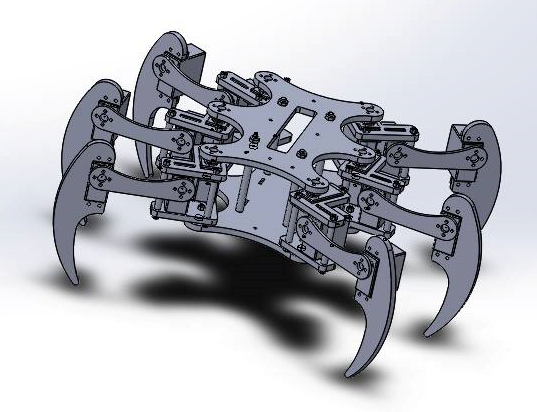
\includegraphics[width =0.8\textwidth]{Fig1}
	\caption{ CAD rendering of the robot.}
	\label{CAD}
\end{figure}
To further develop the kinematic model of the robot, the coordinate systems (Cartesian frames \cite{28}) for all parts of the robot need to be identified. Next, the detailed development of such frames is given.
\subsection{Robot body frame}
The origin of the robot base frame will be in the center of the body, structured with Z-axis pointing up, the X-axis positioning right and Y-axis pointing forwards with respect to the robot front side as depicted in \ref{Loc}.

\begin{figure}[h]
	\centering
	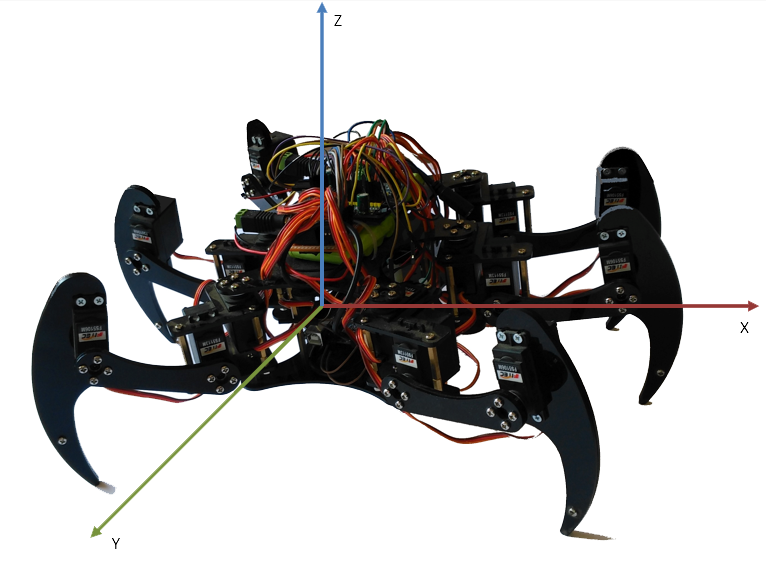
\includegraphics[width =0.8\textwidth]{Fig3}
	\caption{ Location of body frame relative to robot hardware.}
	\label{Loc}
\end{figure}
\subsection{Leg frames and notations}
The design of hexapod constitutes the kinematic configuration of a hexapod robot, with each leg acting as an independent serial manipulator with three degrees of freedom. Figure \ref{fig1} shows the actual prototype of our robot.

\begin{figure}[h]
	\centering
	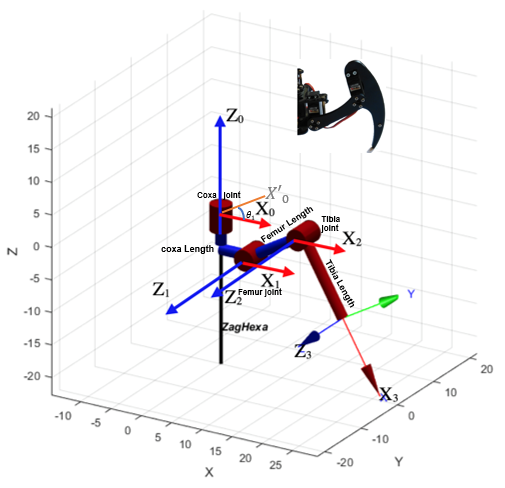
\includegraphics[width =.8\textwidth]{fream}
	\caption{  Final leg design (top right) and its notations, reference frames, joints and links.}
	\label{fream}
\end{figure}

The final leg design and its links and joints notations are given in \ref{fream}. The robot leg is made of links and joints as noted on \ref{leg}, different links of robot leg are called Femur, Tibia and Tarsus. As depicted in figure, the robot leg frame starts with link 0, which is the point where the leg is attached to the body, link 1, is Femur, link 2 is the Tibia and link 3 is Tarsus. The joints are located at the inner end of their respective link. Frames are attached to outer end of their respective links, this means that joint 2 rotates about the Z-axis of frame 1.

\begin{figure}[h]
	\centering
	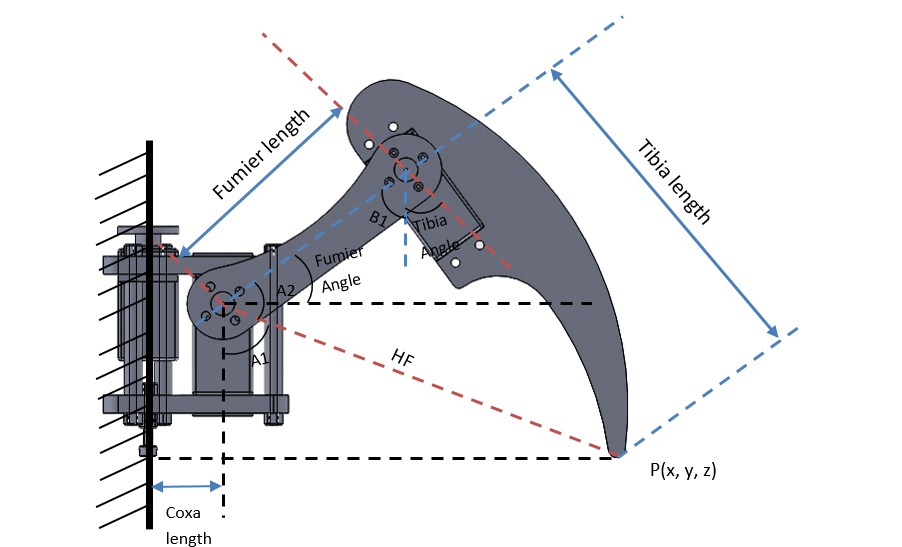
\includegraphics[width =.8\textwidth]{Fig7}
	\caption{  Final leg design (top right) and its notations, reference frames, joints and links.}
	\label{leg}
\end{figure}

\subsection{Robot Leg Parameters}
Following the well-known Denavit-Hartenberg (DH) notation, coordinate frames for the robot leg are assigned. The assigned frames are shown in \ref{leg}. In figure, the body {b} and the zeroth {0} reference frames are attached to the stationary robot body. Therefore, they can be both considered as inertial frames. The axes of the body frame are arranged to be in accord with the actual robot-body orientation. The DH link parameters based on \ref{leg} are given in Table II.\\

The resulting homogeneous transformation matrices between the body and the zeroth frame and between the sequential link frames are given in (1).  In the formulas, the variables represented by $a$ stand for the length of the $i^{th}$ link (namely, the length of the portion of the link between the origins of $(i-1) th and i^{th}$ reference frames). The variables represented by $\theta_{ij}$ mean the sum of the $i^{th}$ and $j^{th}$ joint angles $(\theta_{ij}=\theta_i+\theta_j)$. C and S are for cos(.) and sin(.) functions, respectively.  The exact values of these variables corresponding to ZagHexa robot are: 
$\psi = 45^\circ, a_1= 5cm, a_2= 9cm, a_3= 18cm$
\begin{center}
\begin{tabular}{|c||c|c|c|c|}
	\hline
	Joint & $\theta_i$ & $\alpha_i$ & $a_i$ & $d_i$ \\ \hline
	1&		$\theta_1$ & $\pi/2$	& $a_1$ & 0 \\ \hline
	2&		$\theta_2$ & 0			& $a_2$ & 0 \\ \hline
	3&		$\theta_3$ & 0			& $a_3$ & 0 \\ \hline
\end{tabular}
\end{center}

Homogeneous matrices are used in derivation of positional relations between the successive frames.  In (3) the leg tip point position with respect to the body frame is given. The rotation matrices between the frames are given in (2). These rotation matrices are used in vector equations, especially while deriving the dynamic equations.
\begin{center}

\[
H^{(b,0)}=
\begin{bmatrix}
0 & \cos(\psi) & \sin(\psi) & 0 \\
-1&		0	   & 		0 	& 0\\
0 & -\sin(\psi)& \cos(\psi) & 0 \\
0 &		0	   & 		0 	& 1
\end{bmatrix}
\]
\end{center}

\begin{equation}
H^{(K-1,K)} =
\begin{bmatrix}
\cos\theta_k &-\cos\alpha_k\sin\theta_k &\sin\alpha_k\sin\theta_k &a_k\cos\theta_k\\
\sin\theta_k &\cos\alpha_k\cos\theta_k &-\sin\alpha_k\cos\theta_k &a_k\sin\theta_k\\
0 &\sin\alpha_k &\cos\alpha_k &d_k \\ 
0 &0 &0 &1
\end{bmatrix}
\end{equation}

\begin{align*}
H^{(0,3)} = H^{(0,1)} H^{(1,2)} H^{(2,3)} H^{(b,3)}= H^{(b,0)} H^{(0,3)}
\end{align*}

\begin{center}
	
	\[
	C^{(b,0)}=
	\begin{bmatrix}
	0 & \cos(\psi) & \sin(\psi) \\
	-1&		0	   & 		0 	\\
	0 & -\sin(\psi)& \cos(\psi) \\

	\end{bmatrix}
	\]
\end{center}

\begin{equation}
C^{(K-1,K)} =
\begin{bmatrix}
\cos\theta_k &-\cos\alpha_k\sin\theta_k &\sin\alpha_k\sin\theta_k \\
\sin\theta_k &\cos\alpha_k\cos\theta_k &-\sin\alpha_k\cos\theta_k \\
0 &\sin\alpha_k &\cos\alpha_k \\ 
\end{bmatrix}
\end{equation}
\begin{equation}
P_e^{(K-1,K)} (\theta) =
\begin{bmatrix}
C\psi(a_1S\theta_1+a_2S\theta_1C\theta_2+a_3S\theta_1C\theta{23})+S\psi(a_2S\theta_2+a_3\theta_{23}) \\
-(a_1C\theta_1+a_2C\theta_1C\theta_2+a_3C\theta_1C\theta_{23})  \\
-S\psi(a_1S\theta_1+a_2S\theta_1C\theta_2+a_3S\theta_1C\theta{23})+C\psi(a_2S\theta_2+a_3\theta_{23}) \\
\end{bmatrix}
\end{equation}
To derive the dynamic equations, first the inertia matrices of the links should be determined. Since the $k^{th}$ reference frame is stationary with respect to the $k^{th}$ link, the inertia tensor of the $k^{th}$ link around its center of mass appears to be a constant matrix with respect to the $k^{th}$ reference frame, as in (4). The values used in these formulations belong to the Hexapod robot. The resulting matrices for each link are in the form of (5).
\begin{equation}
\{J_K\}^{(K)} = J_K^{(K)} = J_K
\end{equation}
\begin{equation}
J_K = \begin{bmatrix}
J_{K1} & 0      & 0 \\
0      & J_{K2} & 0 	\\
0      & 0      & J_{K3} 
\end{bmatrix}
\end{equation}


\subsection{Inverse kinematics}
The forward kinematics (FK) is a simple equation used to calculate the position of the end effectors for the leg in the robot base frame, by injecting values of each joint angle. But the reverse operation, namely inverse kinematics (IK), is more complex. IK is employed to find all the joint angles given the position of the end effectors. In general, solving the IK equations can be a bit of a challenge. Some positions cannot be reached at all, as the physical system is unable to get there, and some end effectors positions can have more than one solution, and not all of them are desirable.

We solve the IK problem for each leg separately, as this makes it possible to solve it geometrically, by setting up some constrains. The first constraint for solving the IK equations due the fact that all robot joints allow rotation about one axis only. The second constraint is that the Femur, Tibia joints always rotate on parallel axes. The third set of constraints arises from the physical limitations for each joint, giving us some angular interval for each joint in which the servos can actually rotate the link. In \ref{leg}, the angles of movement are shown.
First, the coxa angle can be found directly by knowing the end effectors position then simply using $atan2(y,x)$ to calculate it. Equations (6) through (14) are used to find the individual joint angles.
\begin{figure}[h]
	\centering
	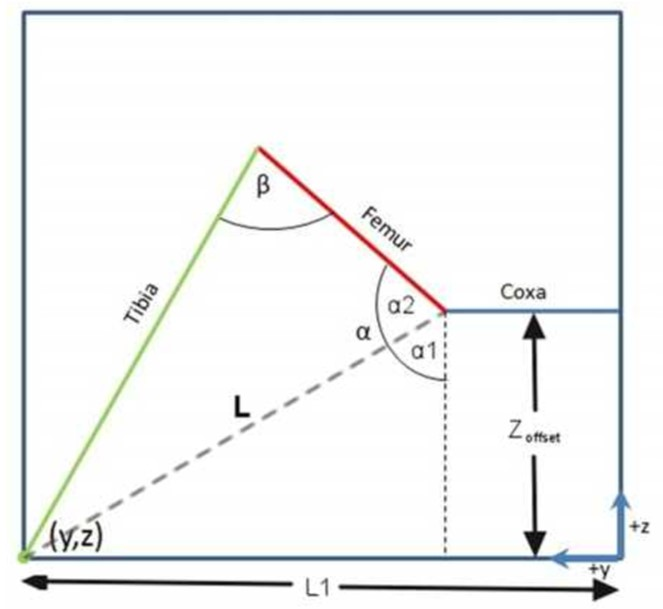
\includegraphics[width =.6\textwidth]{Fig8.jpg}
	\caption{ Illustration of the 2D triangle with vertices in the coxa, the femur, and tibia link from origin.}
	\label{fig8}
\end{figure}

\begin{align}
    \frac{x}{y} & =\tan (y)\to \gamma =\tan ^{-1}\frac{x}{y} \\
    L              & = \sqrt{Z_{offset}^{2}+(L_{1}+\cos A)^{2}}\\
    a_{L}        & = \cos ^{-1}(\frac{Z_{offset}}{L})\\
    Tibia^{2}  & =Femar^{2}+L^{2}-2(Femar)(L)\cos \alpha _{2} \\
    \alpha _{2} & =\cos^{-1}(\frac{Tibia^{2}-Femar^{2}-L^{2}}{-2(Femar)(L)}) \\
    \alpha      & =\alpha _{1}+\alpha _{2}\\
    \alpha      & = \cos ^{-1}(\frac{Z_{offset}}{L})+\cos ^{-1}(\frac{Tibia^{2}-Femar^{2}-L^{2}}{-2(Femar)(L)}) \\
    \beta        & = \cos^{-1}(\frac{L^{2}-Femar^{2}-Tibia^{2}}{-2(Femar)(Tibia)}
\end{align}


\section{Walking Pattern}
In this section, the generation of the robot gait will be described. We provided the robot with a group of programmed gait sequences used for different purposes. For example, a Tripedal gait is used as the basic movement for the robot which provide speed and longer traverse length. Metachronical gait is used for rough terrain traverse which provide better stability but slower motion \cite{29,31}. Main types of gaits used in ZagHexa robot are shown in \ref{walking}. The description of these gaits is given next.
\subsection{Wave gait (Metachronical Gait)}
In this gait mode, the robot move one leg at a time, it starts by lifting one leg and then lowering it down gradually until the foot touches the ground and then the next leg starts to move, as mentioned before this gait sequence is rather slow but it provides maximum stability for the robot, and it enables the robot to walk on rough terrain. This is illustrated in \ref{walking}.

\subsection{Ripple gait (Two wave Gait)}
In this gait, two legs move at a time, since it has two independent wave gaits. The opposite sides legs are 180 degrees out of phase and it needs three beats to complete one cycle. \ref{walking}. shows the Ripple gait.

\subsection{Tripedal Gait}
This gait is the fast gait for the hexapod; it completes a cycle in two beats. In this gait, the robot lift three legs simultaneously while leaving three legs on the ground, which keeps the robot stable. \ref{walking}. shows Tripedal gait reaction \cite{19}.
\begin{figure}[h]
	\centering
	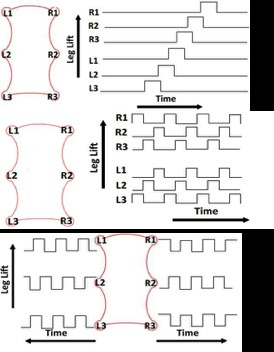
\includegraphics[width =.6\textwidth]{walking}
	\caption{ Different walking gaits: wave (top), ripple (middle), and tripod (middle).}
	\label{walking}
\end{figure}